\begin{coverpages}
{
\renewcommand\labelitemi{$\vcenter{\hbox{\tiny$\bullet$}}$}
\setlist[itemize]{
    itemsep=-1em,
    align=parleft,
    leftmargin=1em,
    labelwidth=0.5em,
    topsep=0em
}
    \begin{minipage}{0.25\linewidth}
        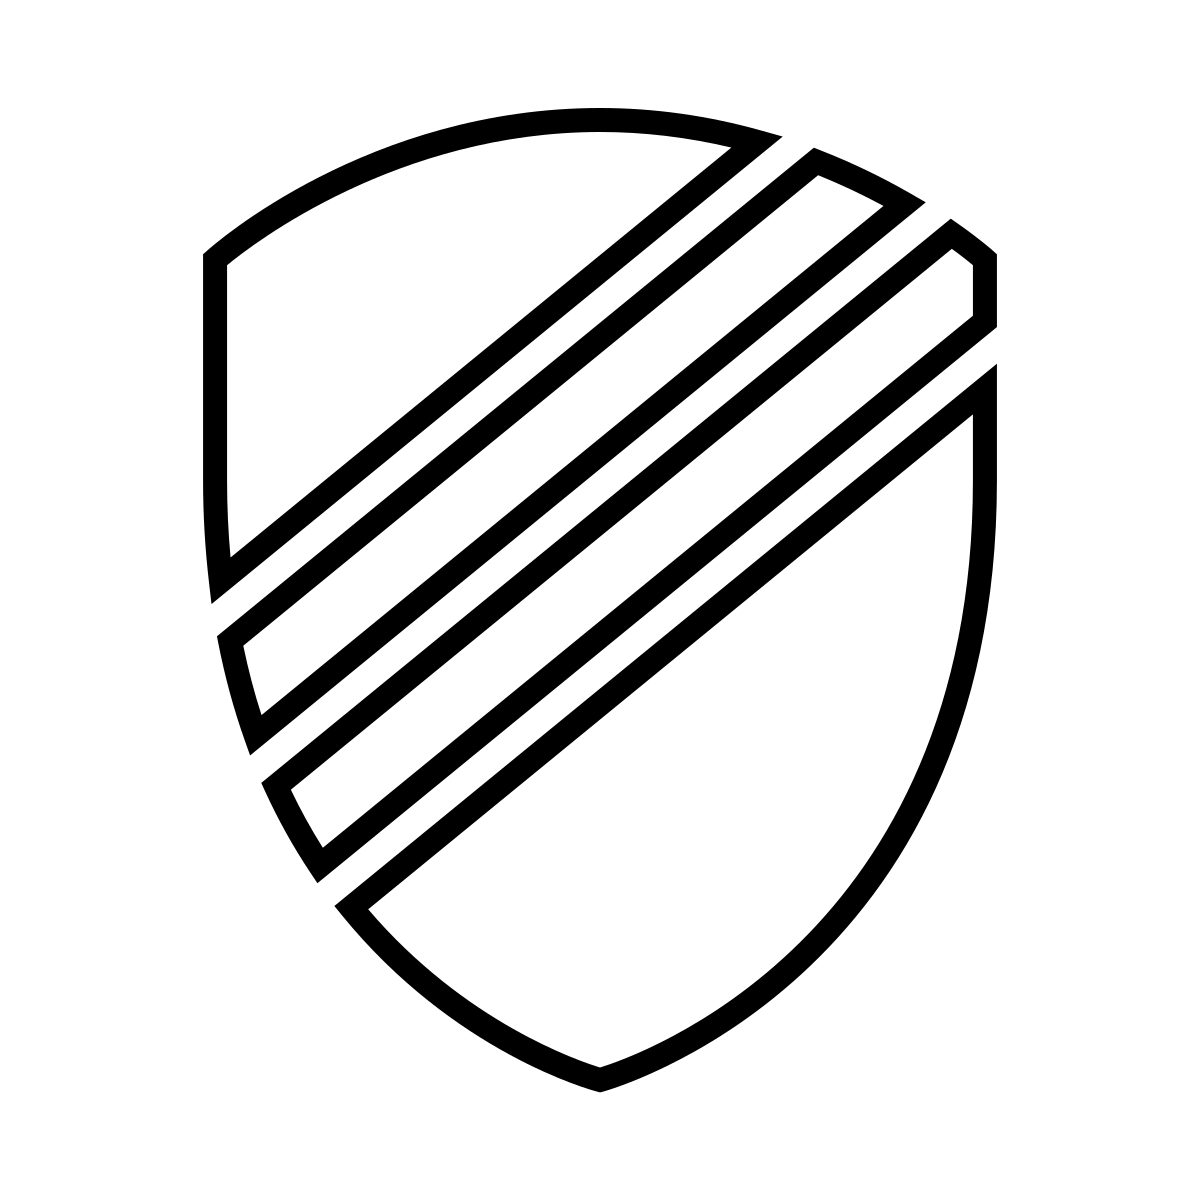
\includegraphics[width=2.9cm]{include/crest.png}
    \end{minipage}
    \begin{minipage}{0.7\linewidth}
        \begin{flushright}
        {\large
            School of Rock\\\vspace{1ex}
            Mathematics Department\\\vspace{1ex}
            Specialist Mathematics\\\vspace{1ex}
            \the\year{}\\\vspace{1ex}
            Task 1\\\vspace{1ex}
        }
            \end{flushright}
    \end{minipage}
    
    \vspace{1cm}    % vertical space
    \textbf{Question booklet}
    \begin{itemize}
        \item Answer \textbf{\textit{all}} questions
        \item Write your answers in this question booklet
        \item Allow approximately 70 minutes
        \item Approved calculators may be used
    \end{itemize}
    \vfill
    \textbf{Examination information}\par
    \textbf{Materials}
    \begin{itemize}
        \item Question booklet
        \item Formula sheet
    \end{itemize}
    \textbf{Instructions}
    \begin{itemize}
        \item Show appropriate working and steps of logic in the question booklets
        \item State all answers correct to three significant figures, unless otherwise instructed
        \item Use black or blue pen
        \item You may use a sharp dark pencil for diagrams
    \end{itemize}
    \textbf{Total time:} 70 minutes\\
    \textbf{Total marks:} 60
    \vfill
    Student Name:\ \parbox[b][2em][b]{6cm}{\dotfill}
    \hfill
    Teacher:\ \parbox[b][2em][b]{5cm}{\dotfill}
    
%\coverlfoot{Student Name:\ \parbox[b][2em][b]{6cm}{\dotfill}}
%\coverrfoot{Teacher:\ \parbox[b][2em][b]{5cm}{\dotfill}}
}
\end{coverpages}
\addtocounter{page}{1}

%\blankpage